\documentclass[11pt,a4paper]{report}
\usepackage[T1]{fontenc}
\usepackage[utf8]{inputenc}
\usepackage{lmodern}
\usepackage[french]{babel}
\usepackage{fullpage}
\usepackage{listings}
\usepackage{graphicx}
\usepackage{hyperref}


\title{Projet de SQL: Game of Trones}
\author{Jeremy Wagemans \and Philippe Dragomir}
\date{\today}

\begin{document}
    \lstset{
        tabsize=2,
        basicstyle=\footnotesize,
        frame=single,
        breaklines=true,
        literate=
            {é}{{\'e}}1
            {è}{{\`e}}1
            {ô}{{\^o}}1
            {ê}{{\^e}}1
            {ç}{{\c{c}}}1
            {à}{{\`a}}1,
    }

\maketitle

\addcontentsline{toc}{chapter}{Table des mati\`eres}
\tableofcontents

\begingroup
\setlength{\parskip}{\baselineskip}
\chapter{Introduction}


\begin{flushleft}
Afin d’appliquer les méthodologies et les notions enseignées au cours \href{http://ecampus.ipl.be/claroline/course/index.php?cid=2BIN_SQL}{I2040 - DB : Langage de Requêtes et de Programmation}, nous avions pour objectif de réaliser, par groupe de deux, une application de gestion de devis.
\par
En effet, l'objectif du projet était d'informatiser le processus de soumission et d'acceptation des devis pour les maisons de WCrhoo et de leurs clients. Ils nous ont donc demandés de mettre en place une plateforme permettant de regrouper les demandes de devis des clients et permettant aux différentes maisons de pouvoir soumettre des devis à ces demandes.
\par
La solution qui vous est présentée ci-après est celle du groupe composé de Dragomir Philippe et de Jeremy Wagemans.
\par
Au terme du projet, nous avons donc dû délivrer une solution en parfaite adéquation avec les demandes des maisons et des clients répondant à des critères de qualité stricts. Ce rapport permet donc d’exposer de manière précise son fonctionnement. Il est structuré comme suit:
\par
Dans un premier temps, nous développerons l'interprétation que nous avons faite des demandes des maisons ainsi que de celles des clients.
\par
Ensuite, nous vous exposerons la structure de la base de données crée pour répondre aux demandes énoncés.
\par
Enfin, nous proposerons le code source commenté des deux applications développées.
\end{flushleft}

\endgroup

\setlength{\parskip}{\baselineskip}
\chapter{Présentation de la solution}
\section{Clarification de l'interprétation de l'énoncé}
Certains points du cahier des charges ont été approfondis lors la réalisation du projet, il est donc nécessaire de clarifier les détails suivants:
\begin{itemize}\renewcommand{\labelitemi}{$\bullet$}
  \item Les options sont réutilisables. Une maison peut à tout moment créer et modifier des options. Elle
  peut joindre celles-ci à n'importe quelle offre.
  \item Toutes les statistiques demandées sont précalculées mis à part le nombre de devis en cours. En effet, vu que le système de gestion
  de bases de données ne sait pas gérer la notion d'expiration temporelle de manière systématique, il est nécessaire de recalculer ce nombre à chaque fois qu'on en a besoin.
  \item Lorsqu'une maison est dénoncée, le devis dénonciateur est transformé en un devis normal, c'est-à-dire non masquant et publique.
\end{itemize}

\newpage
\section{Structure de la base de données}
\begin{flushleft}
Les données de l’application sont sauvegardées dans une base de données, structurée comme suit :
\begin{center}
  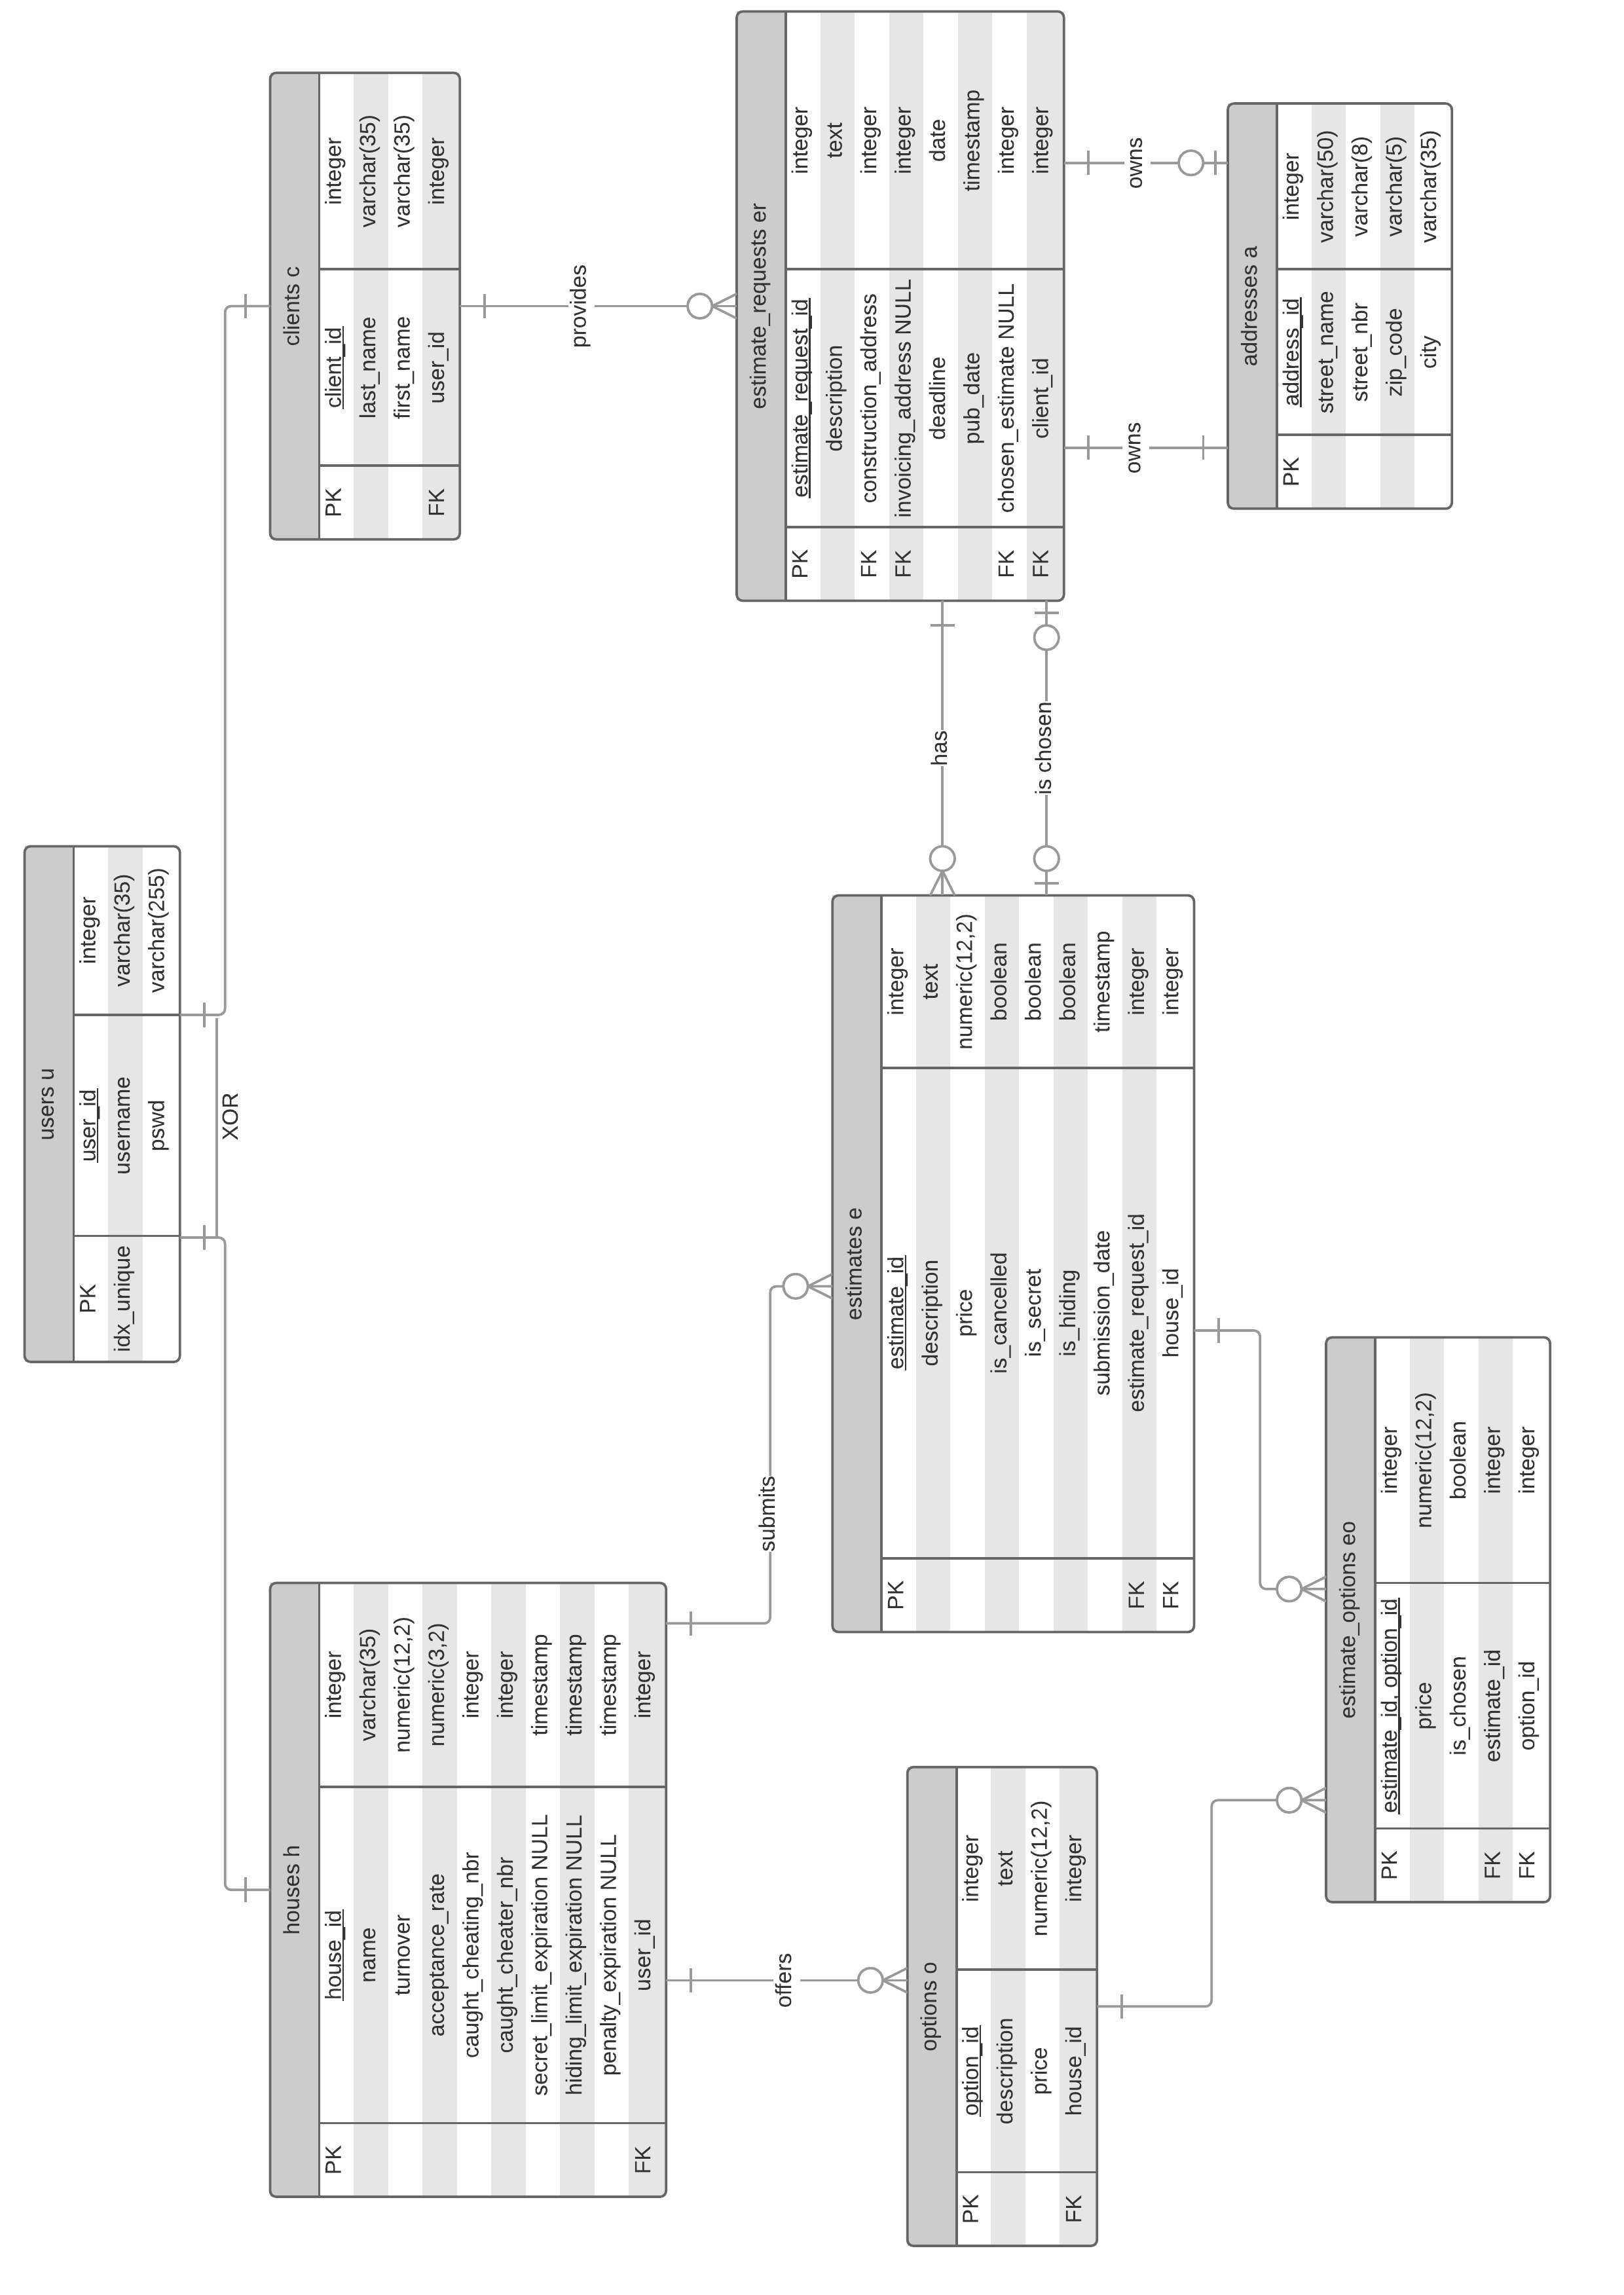
\includegraphics[scale=0.65]{dsd.png}
\end{center}
\end{flushleft}

\newpage
Il est essentiel de mentionner certaines spécificités du schéma :

\begin{itemize}\renewcommand{\labelitemi}{$\bullet$}
    \item Un utilisateur représente un client ou une maison autorisé à utiliser l’application et
    est authentifié grâce à un nom d’utilisateur unique et à un mot de passe.
    \item Le fait qu’un devis soit caché et/ou masquant est déterminé sur base des champs booléens is\_secret
    (vrai lorsqu’un devis est caché) et is\_hiding (vrai lorsqu’un devis est masquant) de la table estimates.
    \item Un devis est annulé lorsque celui-ci a été soumis dans un délais de 24 heures avant que la maison soumissionnaire ne soit démasquée pour tricherie. Dans ce cas, le champs booléen is\_cancelled de ces devis dans la table estimates vaut vrai.
    \item Le choix d’un devis par le client s’exprime au sein de la table estimate\_requests au travers du champs chosen\_estimate. Celui-ci référencie donc le devis choisi. Si aucun devis n’a encore été accepté, ce champs est vide. Par conséquent, il n’est pas nécessaire de parcourir l’entièreté des devis pour savoir si un devis a été accepté pour une demande et lequel a été accepté.
    \item Le champs pub\_date d’une demande de devis exprime sa date de publication. Une demande est donc expirée lorsque cette date est antérieure à 15 jours.
    \item Les options sont réutilisables. Etant donné que leur prix peut être modifié, le prix d'une option est lié à un devis (table estimate\_options).
    \item Les statistiques pré-calculées sont enregistrées au sein de la table maison.
\end{itemize}


\setlength{\parskip}{0pt}
\chapter{Base de données}

\section{Script d'installation}
\lstinputlisting[language=sql]{../SQL/install.sql}
\newpage

\section{Script d'insertion de données valides}
\lstinputlisting[language=sql]{../SQL/src/insert_valid_data.sql}
\newpage

\section{Script d'insertion de données invalides}
\lstinputlisting[language=sql]{../SQL/src/insert_invalid_data.sql}
\newpage

\chapter{Application java}
\section{App.java}
\lstinputlisting[language=java]{../app/marche_halibaba/src/marche_halibaba/App.java}
\newpage

\section{ClientsApp.java}
\lstinputlisting[language=java]{../app/marche_halibaba/src/marche_halibaba/ClientsApp.java}
\newpage

\section{HousesApp.java}
\lstinputlisting[language=java]{../app/marche_halibaba/src/marche_halibaba/HousesApp.java}
\newpage

\section{Utils.java}
\lstinputlisting[language=java]{../app/marche_halibaba/src/marche_halibaba/Utils.java}
\newpage

\section{PasswordHash.java}
\lstinputlisting[language=java]{../app/marche_halibaba/src/marche_halibaba/PasswordHash.java}
\newpage

\setlength{\parskip}{\baselineskip}
\chapter{Conclusion}
\begin{flushleft}
A l’issue d’un mois de travail intensif, nous pouvons affirmer que ce projet s’est terminé sans encombre et dans les délais.
Nous avons atteint les objectifs que nous nous sommes fixés initialement et avons réalisé une solution répondant parfaitement au cahier des charges.
\par

Nous estimons la période de réalisation de l’entièreté de l’application à 50 heures réparties comme suit:
5h pour l’analyse, 30 heures pour la conception de la base de données et 15h pour le développement de l’application java.
\par

Nous avons eu l’opportunité, grâce à ce projet, d’améliorer et d’approfondir nos connaissances en SQL ainsi qu’à nous familiariser aux bonnes pratiques de jdbc, le driver SQL pour java.
Nous avons également pu appliquer l’ensemble des savoir-faire acquis en cours de conception de bases de données.
\par

Du point de vue humain, il nous a permis d’apprendre à mieux nous connaître.
Nous avons appris à travailler ensemble de manière efficace en répartissant la charge de travail selon nos forces et faiblesses.
\par

C’est donc pleinement satisfaits que nous délivrons ce projet aujourd’hui.
\end{flushleft}
\end{document}
